\section{Validation and Results}
\label{sec:results}

\subsection{Regression Suites}

Every layer has a self-verifying suite (Table~\ref{tab:suites}); all
pass at the state documented here, and the counts below were taken
from a run of each at the time of writing rather than copied forward.
The suites fall into three groups: the Python model against the
article and against itself, the C implementation against golden
vectors the Python model generates, and the hosts against the
device-side C running as a process.

\begin{table}[H]
    \centering
    \caption{Verification suite summary.}
    \label{tab:suites}
    \small
    \begin{tabular}{@{}lrp{7.6cm}@{}}
    \toprule
    \textbf{Suite} & \textbf{Checks} & \textbf{Scope} \\
    \midrule
    \multicolumn{3}{@{}l}{\textit{Python model}} \\
    \texttt{verify\_article.py} & 44 & bit-exact article worked examples:
        CRCs, Base38/QTH, conv-code outputs at all rates,
        scrambler/interleaver sequences, ZC ACF
        (Appendix~\ref{app:verify}) \\
    \texttt{smoke\_e2e.py}      & 13 & end-to-end TX$\to$channel$\to$RX
        incl.\ CFO, all modes, STF, auto-mode detection \\
    \texttt{fixed\_point.py}    & 28 & fixed-point primitives, TX/RX
        parity, LDPC and 16-QAM TX and RX, HARQ, calibration, SNR
        estimator and its output map (Appendix~\ref{app:fixed}) \\
    \texttt{rf\_channel.py}     &  6 & SSB transparency, LO-derived CFO
        to 0.1\,Hz, decode through the fading RF chain \\
    \texttt{afc\_netting.py}    & --- & netting convergence +
        trim-budget and anchor guard scenarios (PASS/FAIL) \\
    \texttt{simplex\_session.py}& --- & whole-system two-station test,
        bit-exact delivery assert (PASS/FAIL) \\
    \midrule
    \multicolumn{3}{@{}l}{\textit{C implementation (\texttt{make -C cport test})}} \\
    \texttt{test\_primitives}   & 11 & FFT, Hilbert, NCO, CORDIC against
        the fixed-point ROMs \\
    \texttt{test\_bits}         & 16 & CRC, FEC, puncturing, interleaver,
        scrambler, LDPC \\
    \texttt{test\_tx}           & 15 & frames and bursts against golden
        hashes, all modes and modulations \\
    \texttt{test\_rx}           & 22 & detection and demodulation
        against genie vectors, two-lag unwrap, SNR map \\
    \texttt{test\_stream}       & 11 & streaming receiver: chunked
        feeding, burst continuation, block-aligned leads, the
        weak-spike soak seed \\
    \texttt{test\_link}         & 80 & controller, station, ARQ, bursts,
        capability handshake, operator ceilings, codec bitmap,
        sentinel codes \\
    \texttt{test\_broadcast}    &  4 & group build and walk \\
    \texttt{test\_usb}          & 18 & framing, parser resync, structure
        round trips and grow-only decoding \\
    \texttt{make robust}        & --- & \texttt{burst\_repro} abuse matrix,
        \texttt{bc\_repro}, \texttt{bc\_soak}, \texttt{cstest}
        (Section~\ref{sec:chan_harness}); \texttt{make sanitize-ship}
        runs the suites under ASan/UBSan at the shipping geometries \\
    \midrule
    \multicolumn{3}{@{}l}{\textit{Hosts}} \\
    \texttt{host/test\_ofdm\_modem.py} & 11 & driver against the
        device-side C on stdio \\
    \texttt{host/test\_modem.py}       &  7 & driver in isolation: serial
        retry, langid cache, payload cap \\
    \texttt{host/test\_kiss.py}        & 41 & KISS codec, air-time
        admission table never optimistic \\
    \texttt{host/test\_ip\_tun.py}     & 32 & tunnel queueing policy \\
    \texttt{demoapp/test\_board\_console.py} & --- & file envelope
        offsets, window-aligned splitting \\
    \bottomrule
    \end{tabular}
\end{table}

\subsection{Article Reproduction}

\begin{table}[H]
    \centering
    \caption{Reproduction versus the article.}
    \label{tab:reproduction}
    \small
    \begin{tabular}{@{}lll@{}}
    \toprule
    \textbf{Metric} & \textbf{Article} & \textbf{This implementation} \\
    \midrule
    Worked examples & --- & 44/44 bit-exact \\
    Sensitivity, BPSK 1/3 & $\approx -7.5$\,dB &
        $-7.2$\,dB raw RX; $-7.6$\,dB genie-synchronized \\
    BER/PER curves (Figs.~23--24) & simulated &
        reproduced (Figure~\ref{fig:berper}), both preambles \\
    \bottomrule
    \end{tabular}
\end{table}

The remaining 0.3\,dB between the raw and genie-synchronized receiver
is residual synchronization loss at low SNR (occasional missed
detections and one-symbol timing slips), not the decode chain ---
i.e.\ the reproduction gap is closed to within measurement noise of
its diagnosed cause.

\begin{figure}[H]
    \centering
    \begin{subfigure}{0.49\textwidth}
        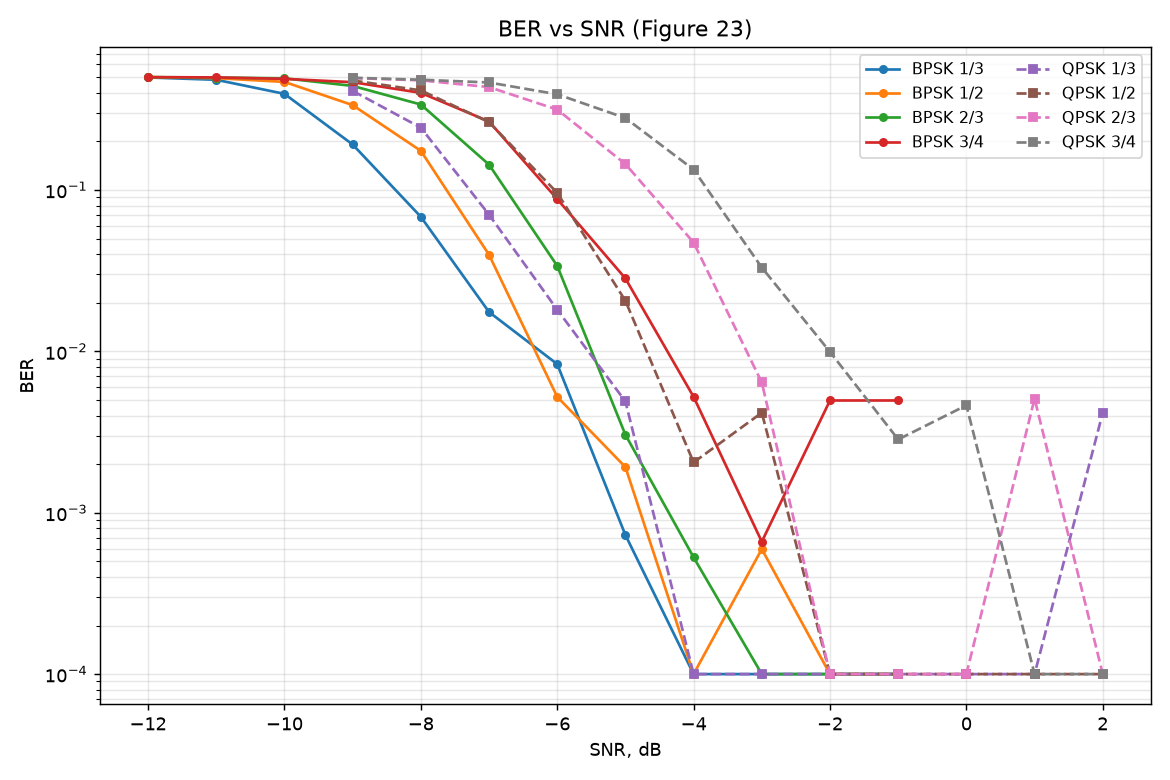
\includegraphics[width=\textwidth]{images/ber_vs_snr.png}
        \caption{BER versus SNR.}
    \end{subfigure}
    \hfill
    \begin{subfigure}{0.49\textwidth}
        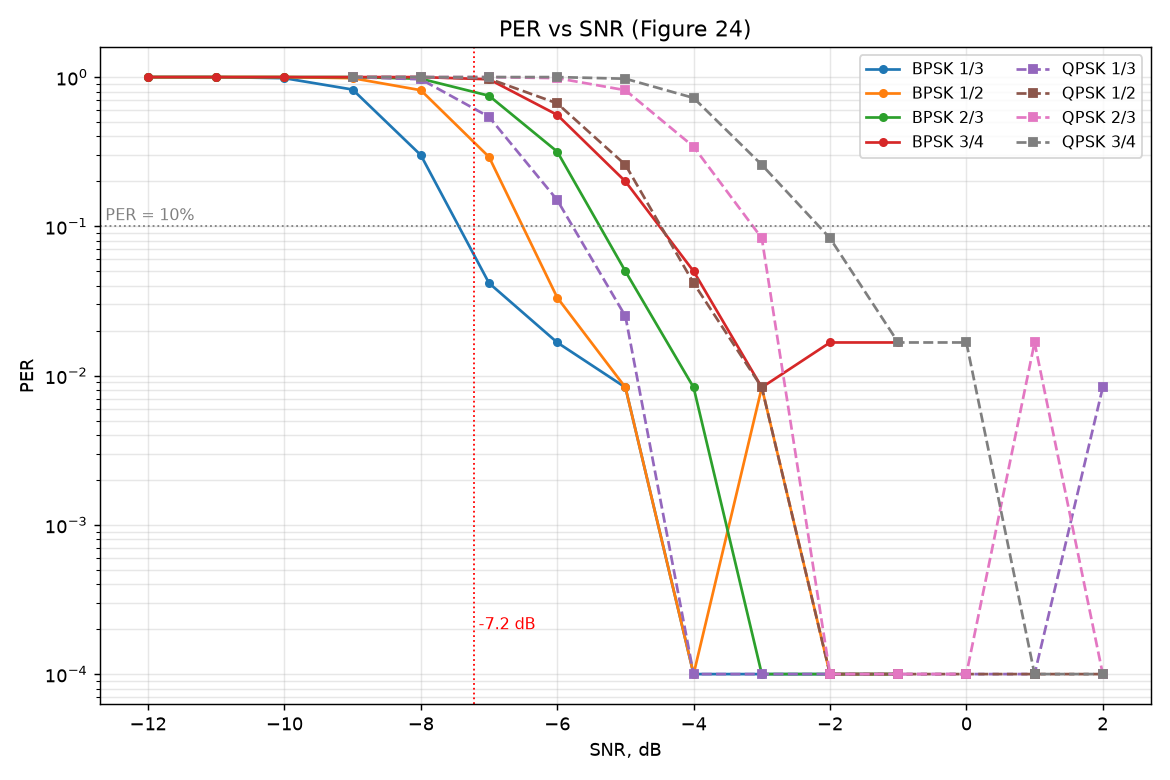
\includegraphics[width=\textwidth]{images/per_vs_snr.png}
        \caption{PER versus SNR.}
    \end{subfigure}
    \caption{Reproduction of the article's Figures~23--24: eight
             modulation/rate configurations over the article channel
             model (multipath $[1,0,0.4,0,0,0.2]$, BSC $10^{-3}$, BEC
             $2\cdot 10^{-2}$, random $\pm 100$\,Hz CFO with drift,
             random timing), 120 packets per point.}
    \label{fig:berper}
\end{figure}

\begin{figure}[H]
    \centering
    \begin{subfigure}{0.49\textwidth}
        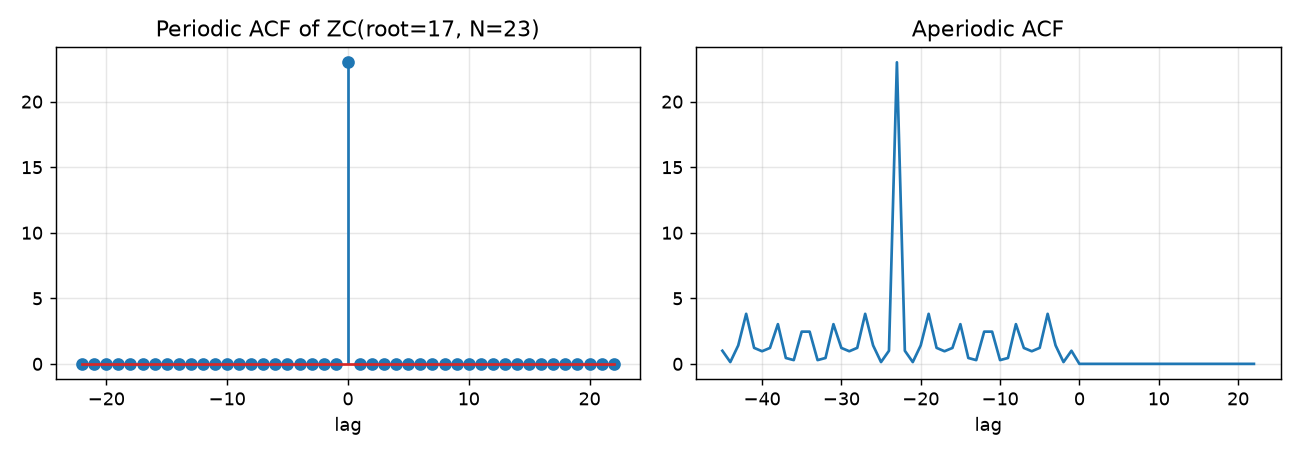
\includegraphics[width=\textwidth]{images/zc_acf.png}
        \caption{Zadoff--Chu autocorrelation.}
    \end{subfigure}
    \hfill
    \begin{subfigure}{0.49\textwidth}
        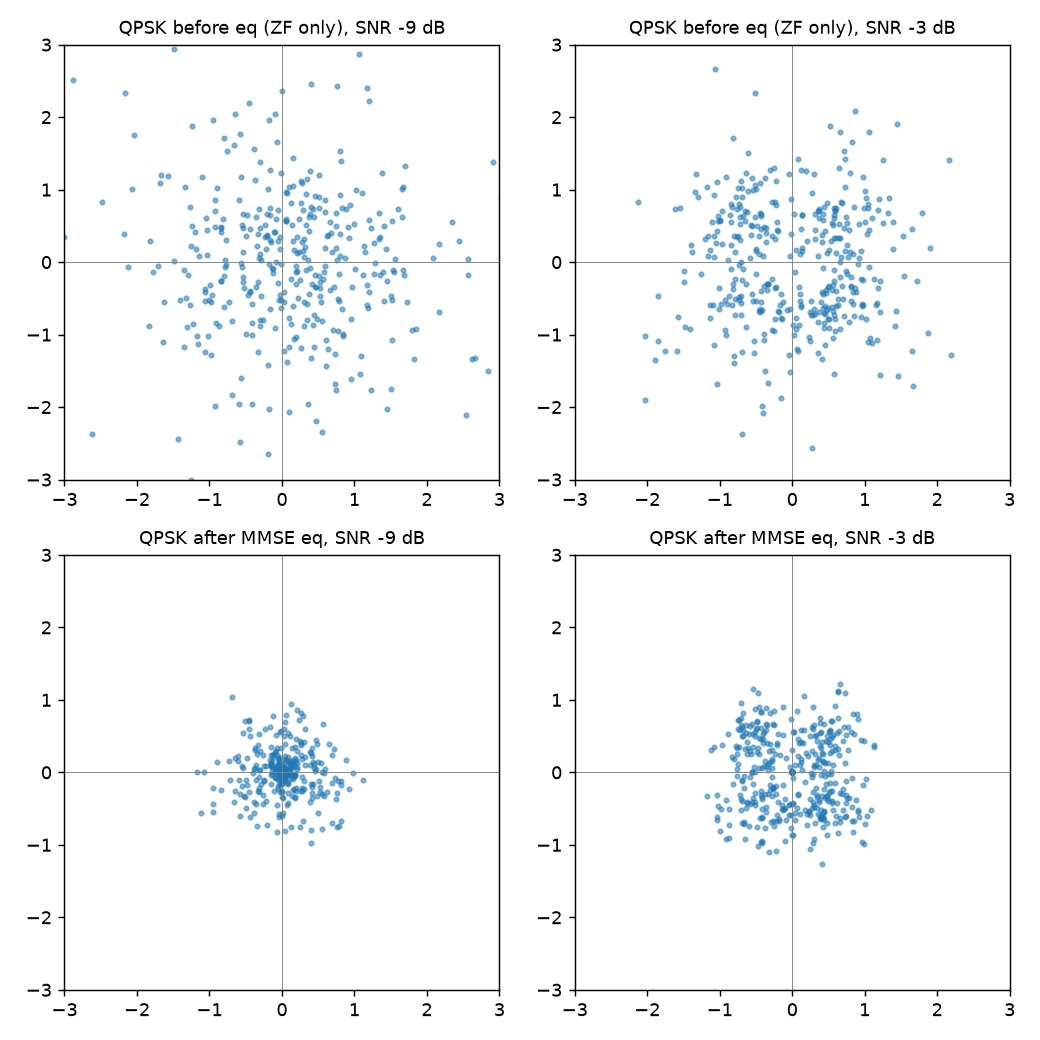
\includegraphics[width=\textwidth]{images/constellation_qpsk.png}
        \caption{QPSK constellation, before/after equalization.}
    \end{subfigure}
    \caption{Article-style diagnostic figures
             (\texttt{experiments/figures.py}).}
    \label{fig:diag}
\end{figure}

\subsection{Measured Feature Gains}

Table~\ref{tab:gains} consolidates every A/B-measured improvement.
All A/B comparisons use paired channel realizations
(Section~\ref{sec:conventions}); sensitivity points use 40--300
trials; the board-side rows are measured on the wire stand or the
harness named in their section.

\begin{table}[H]
    \centering
    \caption{Feature gains, A/B measured.}
    \label{tab:gains}
    \small
    \begin{tabular}{@{}p{4.6cm}p{9.6cm}@{}}
    \toprule
    \textbf{Feature} & \textbf{Measured effect} \\
    \midrule
    LLR recalibration & $+1.5$--2\,dB on BPSK/QPSK rungs ($-9$\,dB:
        6/40 $\to$ 29/40); regresses 16-QAM $\to$ gated to
        $\mu \le 2$ \\
    HARQ chase combining & 2nd attempt 15/20 vs.\ 10/20 at
        $-8.5$\,dB (noise-limited regime) \\
    LDPC (IRA 768/256) vs.\ conv & $+0.7$\,dB AWGN at BLER 10\,\%;
        $\approx$ parity end-to-end (front-end LLR quality binds) \\
    STF preamble variant & equal to Newman everywhere ($\pm 0.14$\,dB
        over 8 configs, $2\sigma$ agreement per point) \\
    AFC netting & $+284$\,Hz $\to$ $<12$\,Hz in 5 exchanges; steady
        $\le 11$\,Hz under 0.09\,Hz/s relative drift \\
    Fixed-point RX vs.\ float & $\le 0.5$\,dB loss at $-7$\,dB;
        \emph{ahead} at $-9/-10$\,dB (22 vs.\ 20, 11 vs.\ 5 of 30,
        against float+recal); 16-QAM within 0.3--0.8\,dB after
        per-modulation LLR quantization (8-bit for $\mu = 4$) \\
    Integer SNR estimator & $\le$1.5\,dB error, $-17\ldots+8$\,dB, all
        modes; gain weighting essential (equal-weight pooling was
        5--15\,dB pessimistic on faded EXTREME frames); output map
        brings the twins to $\sim$0.3\,dB of each other \\
    Two-lag CFO unwrap (fixed/C) & recovers $\sim$8\,\% of all
        acquisitions; broadcast delivery 60\,\% $\to$ 87\,\% at
        $-4.5$\,dB, 79\,\% $\to$ 100\,\% at $-3$\,dB \\
    Streamed bursts & $1.73\times$ throughput for 0.08\,dB at NORMAL;
        $1.21\times$ for $\sim$0.35\,dB at EXTREME \\
    Interference: preemption, net key, carrier excision, LLR
        weighting & same-mode stranger frames, C receiver: 10\,\%
        threshold $-8.8 \to -2.6$\,dB and ``never'' $\to -2.4$\,dB (the
        lock-stealing limit); CW carrier: $-4.8 / -4.2$\,dB $\to$ no
        failure up to ISR $+10$\,dB at NORMAL; EXTREME knee identical,
        host cost unchanged, $+44$\,kB RAM \\
    \midrule
    \multicolumn{2}{@{}l}{\textit{C implementation and boards}} \\
    RAM, three-mode receiver & 10\,MB host reference $\to$ 561\,KB
        (bit-exact); 27\,KB transmit-only \\
    Flash & 242\,KB $\to$ 57\,KB, bit-exact \\
    EXTREME frame CPU (STM32H743) & 23.7\,\% $\to$ 9.5\,\% of a
        480\,MHz core; acquisition 8.44\,s $\to$ 2.12\,s inside a
        5.08\,s window; ring 288 $\to$ 160\,KB; $\le$0.01\,dB
        sensitivity cost, 0 false alarms in 250 \\
    ZC-anchor / weak-commit gates & commit gate: 28/720 $\to$ 0/1800
        groups lost on \texttt{bc\_soak}; 24/24 live voice
        transmissions ($\sim$900 frames) with zero loss \\
    Capability handshake + window-aligned parts & 68\,kB over the
        wire: 50 $\to$ 87 $\to$ 102 $\to$ 114\,B/s (87\,\% of the
        rung-12 raw rate), zero retransmissions \\
    Broadcast block statistics under fade & $+32$\,\% (floor $-5$\,dB)
        and $+39$\,\% (floor $-2$\,dB) of the stream delivered vs.\
        a held rung \\
    DC-blind front end & 8\,kB stress transfer 255 $\to$ 241\,s,
        8 $\to$ 5 timeouts; abuse matrix 8/8 rows bare; CS scenario
        suite 7/7 \\
    Voice on the air & first audio 3.6 / 4.8 / 8.5\,s after the
        talker starts (live / balanced / quality); lag drift
        $\le 0.014$\,s per second; GPU decode step 830 $\to$ 148\,ms \\
    \bottomrule
    \end{tabular}
\end{table}

\subsection{Co-channel Interference}
\label{sec:interference}

\texttt{experiments/interference.py} keys a third party over the
channel while one frame is received and sweeps the
interference-to-signal ratio (ISR: the interferer's mean power over
the recording against the frame's power at the channel output).  The
interferers are the same mode's preamble train, another mode's
preamble train, a second link's data frames, synthesised SSB voice
(pitch harmonics through formant resonators under a syllable
envelope, 300--2700\,Hz) and a CW carrier; both the float
frame-at-once receiver and the C streaming receiver see byte-identical
recordings, 60 frames per point, the interferer on for at least one
EXTREME tone field (5.1\,s) before the frame so that the streaming
carrier finder is in steady state.  Table~\ref{tab:interference} gives
the ISR at which PER crosses 10\,\% with the preemption of
\S\ref{sec:tone_stream_preempt}, the excision of \S\ref{sec:excision},
the weighting of \S\ref{sec:iweight} and the net key of
\S\ref{sec:net_key} in place; ``never'' means PER stays under 10\,\%
up to ISR $+10$\,dB.

\begin{table}[H]
    \centering
    \caption{ISR (dB) at PER 10\,\%, float frame-at-once / C streaming receiver.  A lower figure means a weaker stranger already breaks the link.}
    \label{tab:interference}
    \footnotesize
    \begin{tabular}{@{}lccc@{}}
    \toprule
    \textbf{Interferer} & \textbf{NORMAL $\frac12$, $-3$\,dB} & \textbf{NORMAL $\frac12$, $+10$\,dB} & \textbf{EXTREME $\frac13$, $-15$\,dB} \\
    \midrule
    same-mode preamble  & $-5.4$ / $-2.9$ & $-10.0$ / $-2.7$ & $-2.8$ / $-2.7$ \\
    other-mode preamble & $-4.0$ / $-2.6$ & $-9.5$ / $-2.9$ & $-1.0$ / $-2.1$ \\
    same-mode frames    & $-5.4$ / $-2.6$ & $-9.8$ / $-2.4$ & $-2.7$ / $-2.7$ \\
    SSB voice           & $-8.9$ / $-5.8$ & $-10.0$ / $-8.2$ & $-2.2$ / $-2.1$ \\
    CW carrier          & never / never & never / never & never / never \\
    \bottomrule
    \end{tabular}
\end{table}

Against a stranger's preamble train or frames there is still no
margin beyond being the stronger signal: such an interferer breaks the
link within 3--5\,dB of the wanted frame, and at EXTREME within
$\sim$2.5\,dB where it is 15\,dB below the noise, because its tone
comb integrates over the tone field exactly like the wanted one and
steals the lock (the float model's poorer figures at $+10$\,dB on these
rows are the global argmax over a recording that now holds three times
as many stranger preambles).  What changed is everything else.  Before
the four mechanisms the streaming receiver read $-8.8$\,dB and
``never'' (an 18--28\,\% floor from ISR $-20$\,dB up) on same-mode
frames -- a weak stranger's header captured it for a whole data block,
and its CRC-valid frames (25 per minute) fed the ARQ and the ladder --
and both receivers read $-7$ to $-9$\,dB on a CW carrier, which sits
$\sim$17\,dB above the per-carrier signal on its bin, leaks into the
neighbours and, 10\,dB above the signal, blinds the tone detector
outright.  With preemption and the net key the same-mode-frames column
is the lock-stealing limit and nothing else; with the excision a
carrier no longer breaks the link at NORMAL at any ratio measured, and
under a carrier alone the streaming receiver commits once a minute
instead of being blind.  At EXTREME the carrier column first read
$-2.5$\,dB because of a hole at ISR 0\,dB (35\,\% streaming, 53\,\%
float): the first finder counted only the four strongest bins above
$4\times$ per block and found an on-bin carrier but not one split
between two bins; the per-bin finder of \S\ref{sec:excision} closed it
(6.7\,\% at $-3$\,dB, 3.3\,\% at 0\,dB, under 4\,\% everywhere for
both receivers), after the streaming receiver's own two lessons on the
way -- the reset of the search's region when a notch engages, gated on
that region being weak, and a release ratio the finder's sensitivity
can live with.  Voice is unchanged
($-6$ to $-10$\,dB): its harmonics fall on most carriers and its
syllables on half the symbols, so the weighting has no clean reference,
and the detector's lock goes at ISR 0\,dB.  Nothing on the carrier
remains open; the lock-stealing limit and voice do.  The firmware with all four mechanisms runs on the
two-board stand: a 6000-byte file crosses byte-identical in seven frames
each way with no timeouts, the beacons are clean, a mismatched net key
refuses frames on the air (four timeouts in 72\,s) and a matched one
delivers the retransmission at once; the quiet wire's occasional header
attempts predate the campaign, the same captured idle audio committing
identically through the pre-change and current host receivers.

\subsection{The System Demonstration}

The recorded demonstration (\texttt{results/system\_demo.wav},
Figure~\ref{fig:timeline}, transcript in Appendix~\ref{app:demo}) is
the whole system at once: two stations over the fading SSB RF chain
with realistic LO errors, EXTREME-mode negotiation, rate climb,
AFC netting visible in the transcript's CFO column, HARQ, and
bidirectional message transfer --- blind-decoded from the monitor's
audio by \texttt{demod\_frame\_auto} with no side information.
\texttt{experiments/demo\_wav.py} records a complete two-station
session through the RF chain of Section~\ref{sec:rf}: station A at $+6$\,ppm and B at $-8$\,ppm
on 7.1\,MHz (A$\rightarrow$B CFO $\approx +99.4$\,Hz, handled
invisibly by the protocol).  The output WAV is the audio of a
\emph{passive monitor} receiver with its own $+2$\,ppm LO --- A's
frames appear at $\approx +28$\,Hz and B's at $\approx -71$\,Hz in the
blind-decoded transcript (Appendix~\ref{app:demo}), per-station CFO
fingerprints with the thermal drift visible across the session.

\begin{figure}[H]
    \centering
    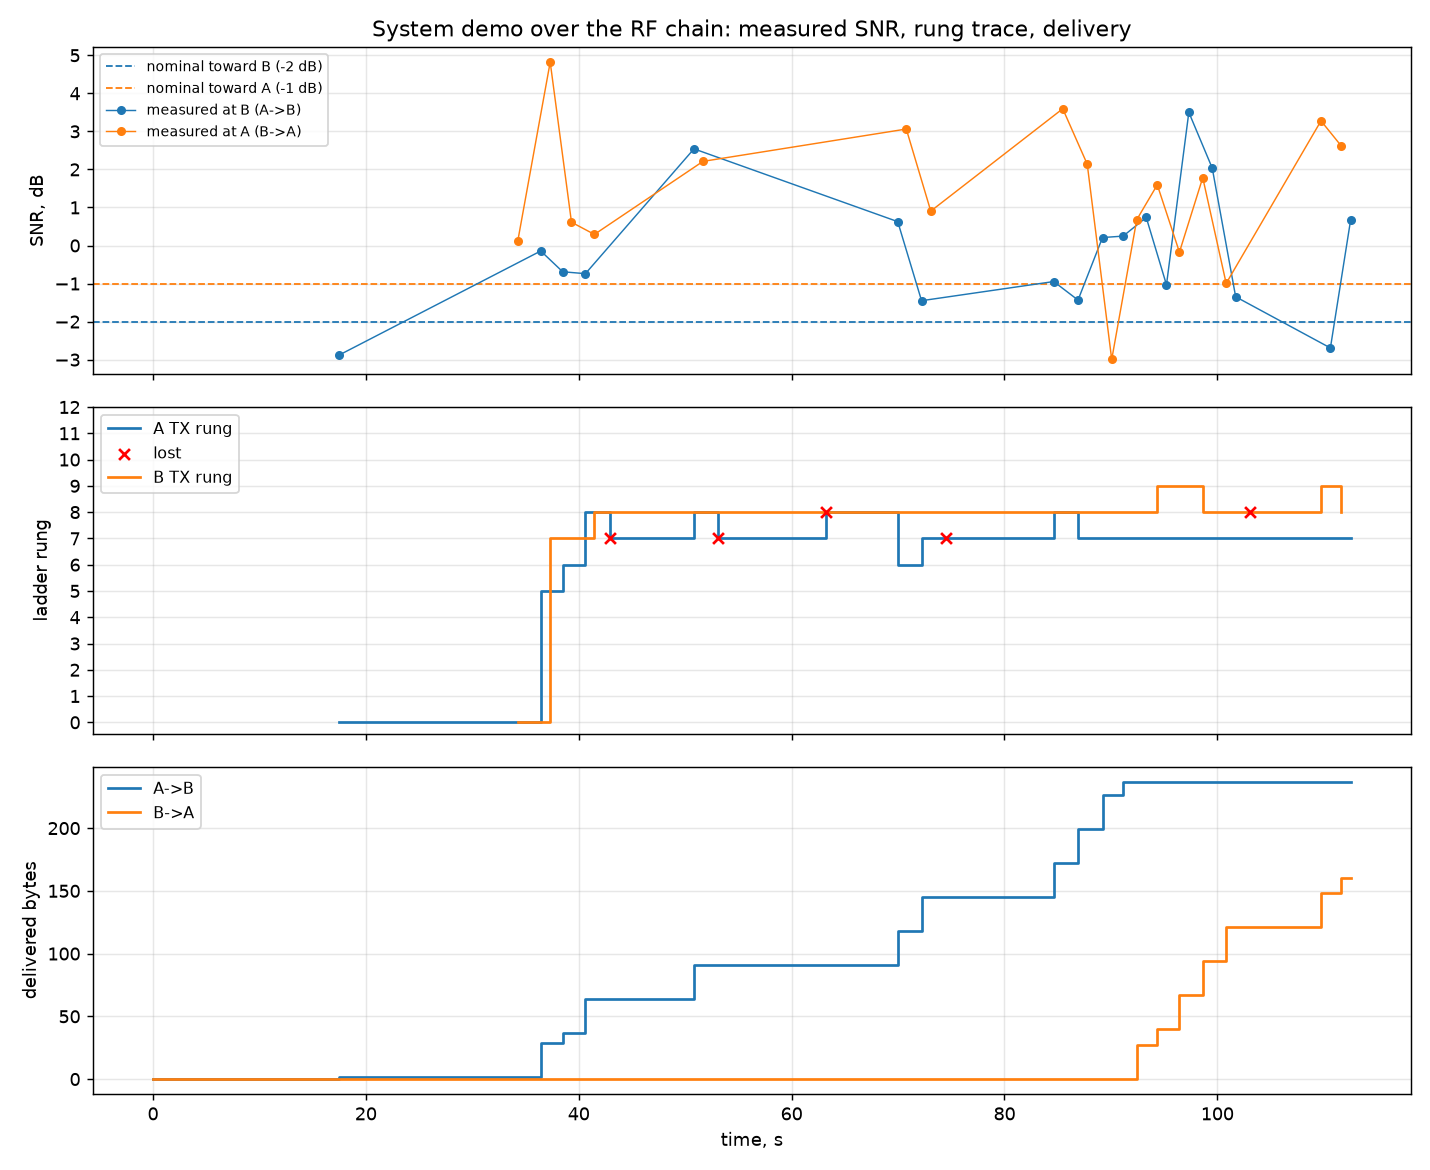
\includegraphics[width=\textwidth]{images/system_demo_timeline.png}
    \caption{System-demo timeline: per-frame SNR, ladder rungs, and
             delivery over the session.}
    \label{fig:timeline}
\end{figure}

The same demonstration also exists on the \emph{fixed-point} pipeline
(\texttt{-{}-phy fixed}, Section~\ref{sec:fixed}): at $-2/-1$\,dB
(\texttt{system\_demo\_fixed.wav}, 37/47 frames blind-decoded) and at
$+5$\,dB, where the ladder climbs into 16-QAM
(\texttt{system\_demo\_fixed\_qam16.wav}, 26/40;
Figure~\ref{fig:fixed_timeline} and Appendix~\ref{app:fixeddemo}).

\begin{figure}[H]
    \centering
    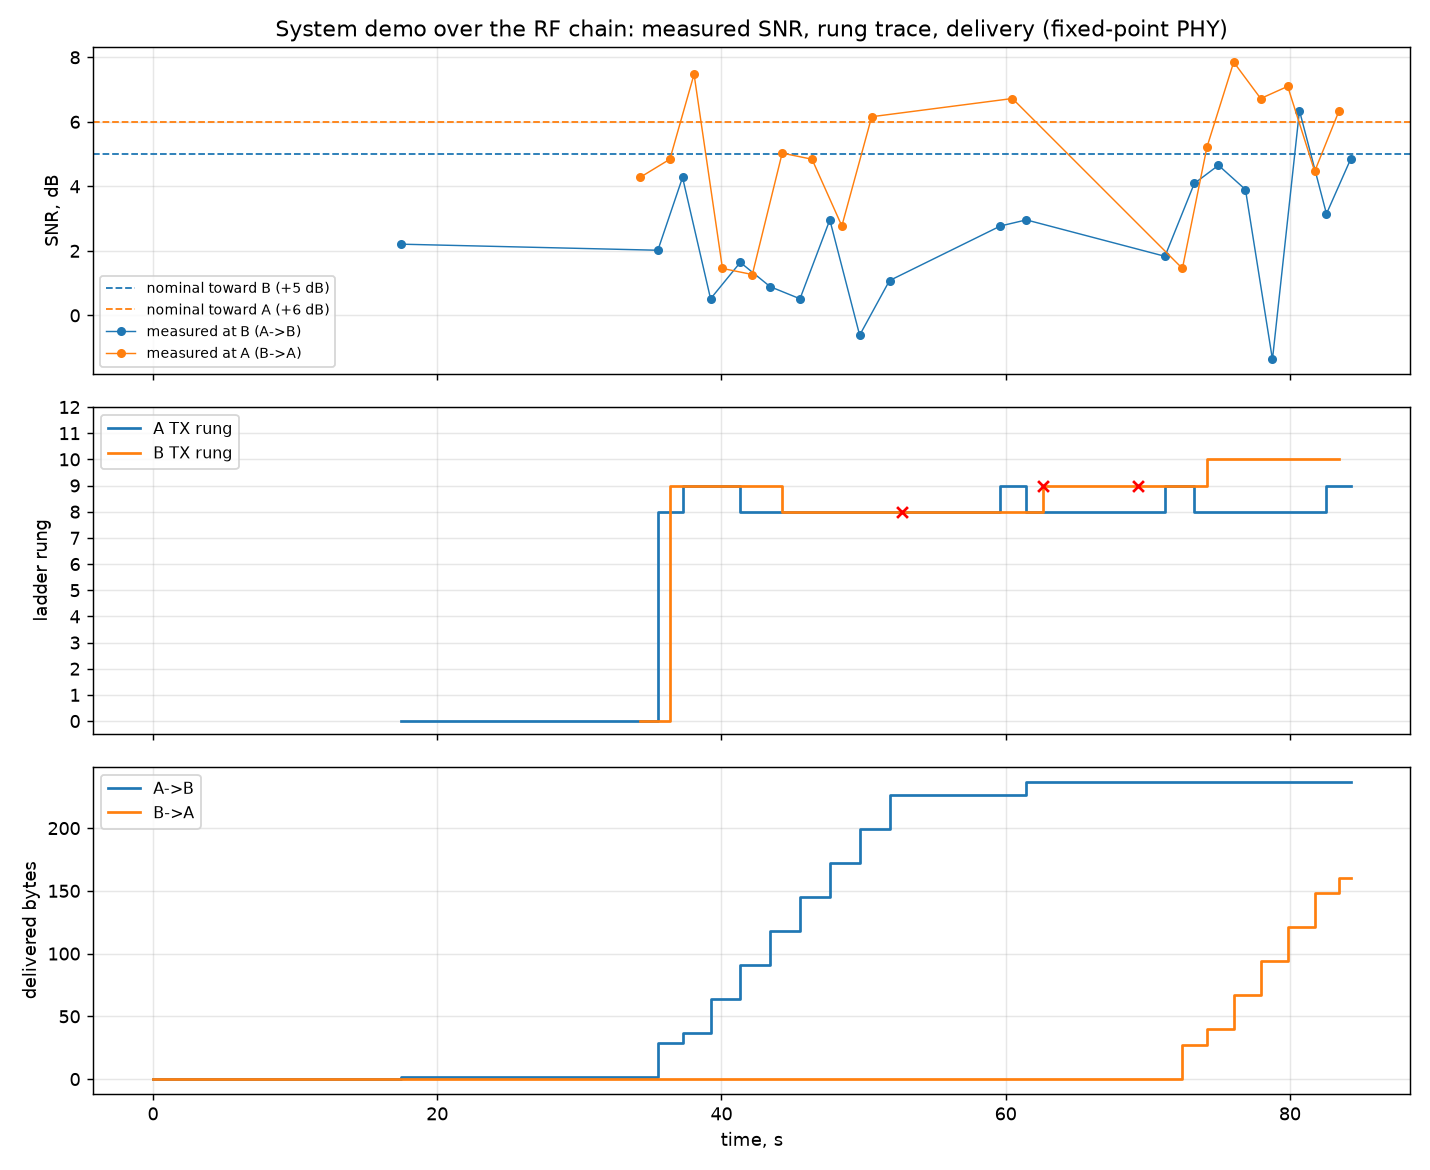
\includegraphics[width=\textwidth]{images/system_demo_fixed_qam16_timeline.png}
    \caption{Fixed-point-pipeline demo at $+5$\,dB: the integer SNR
             estimates drive the ladder into the 16-QAM rungs.}
    \label{fig:fixed_timeline}
\end{figure}

\subsection{Demonstrations on the Boards}

The simulated demonstrations above have physical counterparts, each a
recorded run of Part~\ref{part:impl} on the two-board stand:

\begin{itemize}
    \item \textbf{A file over the acknowledged link} --- a 68\,kB PNG,
          byte-exact in 9.9\,min at rung~12 with the capability
          handshake, window~16 and aligned 3.2\,kB parts
          (\S\ref{sec:cport_levers}); the same file took 25\,min
          before the handshake existed.
    \item \textbf{A file over broadcast} --- 73\,362 bytes in
          22.3\,min at rung~12, 3089 frames, 0 lost, one start event,
          byte-identical (\S\ref{sec:cport_bcast}); and a $-r$~0
          beacon reaching a board that had never exchanged a frame,
          byte-exact at $+16.2$\,dB.
    \item \textbf{An adaptive broadcast} --- 8192 bytes from rung~8,
          re-rung to 12 after the first statistics reply, 350 frames,
          0 lost, a minute faster than the held rung
          (\S\ref{sec:bcstats}).
    \item \textbf{Packet radio and IP} --- a 48-byte AX.25 UI frame
          crossing byte-identical through the KISS bridge in 3.4\,s,
          and a 4\,kB TCP transfer through the tunnel at 43.7\,B/s once
          the queue discipline matched the link
          (\S\ref{sec:cport_kiss}, \S\ref{sec:cport_iptun}).
    \item \textbf{Voice} --- push-to-talk speech at 250\,bit/s over
          broadcast, decoded as it arrives: 24 of 24 transmissions with
          zero loss after the receiver fix, first audio 3.6\,s after
          the talker starts (\S\ref{sec:voice_onair}).
    \item \textbf{Off the air} --- three frames in two modes and two
          modulations recovered over a 7\,MHz RF path through an SDR,
          mode identified from the preamble root alone
          (\S\ref{sec:cport_sdr}).
\end{itemize}

\subsection{Link Budget}

In radio terms, the EXTREME operating point ($-17.5$\,dB planned,
$-17.9$\,dB measured, 6\,kHz reference) needs
$S/N_0 \approx +20.3$\,dB-Hz, i.e.\ $\approx -13.7$\,dB in the
ham-standard 2.5\,kHz bandwidth --- about 7\,dB less sensitive than
FT8~\cite{ft8} and $\sim$20\,dB better than SSB voice.  Against
ITU-R~P.372 noise levels~\cite{itu_p372} with 0\,dBi antennas: on
80\,m at 10\,W, 500--2000\,km reliably on typical nights and
3000--5000\,km from quiet rural sites; on 40\,m at 10\,W,
300--1500\,km all day and worldwide multi-hop on quiet winter nights;
100\,W adds roughly one ionospheric hop to everything.  A planning
caveat: EXTREME's 0.69\,s coherent integration assumes
$\lesssim$0.1\,Hz Doppler spread --- on disturbed or auroral paths
($\ge$1\,Hz) the coherent gain collapses at any power and ROBUST is
the better choice, one more argument for adaptive mode selection.

\subsubsection{Measured Against a Reference Source}
\label{sec:link_budget_measured}

Everything above is derived from a \emph{relative} sensitivity and an
\emph{assumed} noise figure.  With the SDR receiver of
Section~\ref{sec:cport_sdr} on the bench, the assumption can be
replaced by a measurement: a tinySA's calibration output, a reference
tone at a documented level, was fed into the radio through a 40\,dB
attenuator and the receive chain characterised end to end
(\texttt{demoapp/sdr\_rx\_calibrate.py};
\texttt{results/sdr\_rx\_calibration.csv}).  At 10\,MHz with
$-65$\,dBm at the antenna port:

\begin{table}[H]
    \centering
    \caption{Receive chain measured against a reference source
             (HackRF One, LNA 40\,dB).}
    \label{tab:rx_calibration}
    \small
    \begin{tabular}{@{}lp{8.2cm}@{}}
    \toprule
    \textbf{Quantity} & \textbf{Measured} \\
    \midrule
    Frequency error & $-33.1$\,Hz at 10\,MHz $= -3.31$\,ppm, repeatable
                      to 0.0\,Hz ($-23$\,Hz at 7\,MHz) \\
    Linearity       & 1.002\,dB/dB over 16\,dB of gain, 0.03\,dB
                      residual \\
    Receiver noise  & $-95.5$\,dBm in the 6\,kHz reference band
                      (NF $\approx$ 40\,dB) \\
    \midrule
    \multicolumn{2}{@{}l}{\textit{Absolute sensitivity} $=$ measured
      noise floor $+$ the rung's required SNR:} \\
    rung 0 \; EXTREME BPSK 1/3 \; 7.8\,bit/s   & $-113.4$\,dBm \\
    rung 4 \; NORMAL BPSK 1/3 \; 117.6\,bit/s  & $-103.1$\,dBm \\
    rung 12 \; NORMAL 16-QAM 3/4 \; 1059\,bit/s & $-90.8$\,dBm \\
    \bottomrule
    \end{tabular}
\end{table}

Two results matter for planning.  First, the receiver's own noise is
\emph{not} what limits this link: against ITU-R~P.372 atmospheric noise
in the same 6\,kHz band, external noise still dominates by $+9$\,dB at
a quiet rural site, $+17$\,dB at a typical rural one and $+24$\,dB in
residential noise --- so the externally-limited assumption behind the
ranges above holds, and it holds with about 9\,dB of margin at the
quietest sites.  That margin is precisely where a preselector and a
low-noise amplifier begin to pay for themselves, and it is worth noting
that the 40\,dB noise figure measured here belongs to a wideband,
8-bit, unpreselected SDR --- an ordinary HF receiver is far better, so
this is close to a worst case.

Second, the frequency error is negligible for this waveform: 3.31\,ppm
against an acquisition range that tolerates roughly 50\,ppm at 7\,MHz.
A free-running SDR needs no external reference to \emph{acquire} a
frame; a disciplined oscillator matters only for EXTREME's 0.69\,s
coherent integration, where drift \emph{within} a 44\,s frame is the
constraint rather than absolute accuracy.  The absolute levels in
Table~\ref{tab:rx_calibration} inherit the calibration output's nominal
$-25$\,dBm; the relative results --- linearity, frequency error, and
the comparison against atmospheric noise --- do not.

